\documentclass{article}
\usepackage{amsmath}
\usepackage{amsthm}
\usepackage{amssymb}
\usepackage{amsfonts}
\usepackage{mathtools}
\usepackage{listings}
\title{MATH 620: Homework 4}
\author{Fernando}
\date{\today}
\begin{document}
\maketitle
\section*{Problem 1}
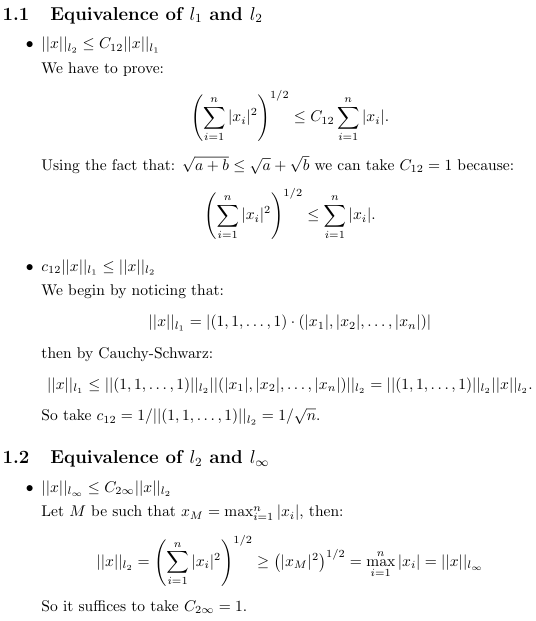
\includegraphics[width=0.99\textwidth]{prob1Part1hw4.png}

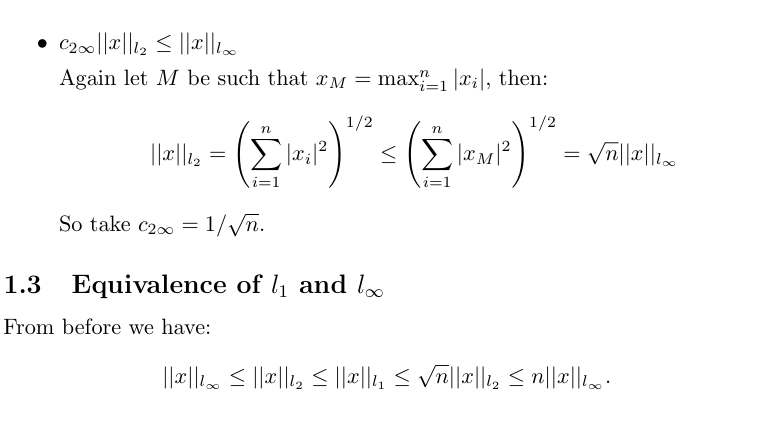
\includegraphics[width=0.95\textwidth]{prob1Part2hw4.png}
\section*{Problem 2}
\subsection*{Norm axioms}
\subsubsection*{$||\cdot||_1$}
All the axioms follow from the properties of the $\max$
\begin{itemize}
\item $\max_{x\in[0.1]}|au(x)|=|a|\max_{x\in[0.1]}|u(x)|$
\item $\max_{x\in[0.1]}|u(x)|=0 \implies \forall x \in [0,1] (|u(x)|\leq 0) \implies u\equiv0$
\item $\max_{x\in[0.1]}|u(x)+v(x)| \leq \max_{x\in[0.1]}|u(x)|+\max_{x\in[0.1]}|v(x)|$
\end{itemize}
The last statement is true because if we find $x_M$ that maximizes the sum $u+v$
then 
\begin{align*}
\max_{x\in[0.1]}|(u+v)(x)|= |(u+v)(x_M)|&\leq|u(x_M)|+|v(x_M)|\\
					&\leq\max_{x\in[0.1]}|u(x)|+\max_{x\in[0.1]}|v(x)|.
\end{align*}
\subsubsection*{$||\cdot||_2$}
Notice that $||u||_2=||u||_1+||u'||_1$. So all the norm requirements follow
from the fact that $||\cdot||_1$ is a norm and that the derivative is linear.
\subsubsection*{$||\cdot||_3$}
In these case the only property that is not immediate is the triangular
inequality. So let's proof that.

By Cauchy-Schwarz:
\[
	\int_0^1|u||v|\leq \left( \int_0^1|u|^2\right)^{1/2} 
	\left(\int_0^1|v|^2\right)^{1/2}
\]
Then:
\begin{align*}
	\int_0^1|u+v|^2&=\int_0^1|u|^2+\int_0^1|v|^2+2\int_0^1uv\\
		&\leq\int_0^1|u|^2+\int_0^1|v|^2+2\int_0^1|u||v|\\
		&\leq\int_0^1|u|^2+\int_0^1|v|^2+2\left(
		\int_0^1|u|^2\right)^{1/2}\left(\int_0^1|v|^2\right)^{1/2}\\
		&=\left(\left(\int_0^1|u|^2\right)^{1/2}+\left(\int_0^1|v|^2\right)^{1/2}\right)^2.
\end{align*}
Taking the square root we obtain the result.
\subsection*{Equivalence of norms}
No two norms are equivalent in this case. Notice that a consequence of the definition of
equivalence of norms is the following:

If $||\cdot||_a$ and $||\cdot||_b$ are equivalent then any sequence that is
convergent in $||\cdot||_a$ must also be convergent to the same limit point in
$||\cdot||_b$. This is because $x_n\to x$ in norm $||\cdot||_a$ means
$||x_n-x||_a\to 0$, and due to the equivalence of norms
\[
	||x_n-x||_b\leq c ||x_n-x||_a
\]
we have
\[
	||x_n-x||_b\to 0.
\]
\subsubsection*{$||\cdot||_1$ vs $||\cdot||_2$}
Since $||u||_2=||u||_1+||u'||_1$ it is clear that convergence in $||\cdot||_2$
implies convergence in $||\cdot||_1$ but the converse is not true.
Pick for example $x_n=x^n/n$. It is easy to see that $x_n\to 0$ in
$||\cdot||_1$ but because $\frac{d}{dx}(x^n/n)=x^{n-1}$ then $||x_n||_2=1$.
So $x_n\nrightarrow 0$ in $||\cdot||_2$. So these norms are not equivalent.
\subsubsection*{$||\cdot||_1$ vs $||\cdot||_3$}
Notice that:
\[
||\cdot||_3^2=\int_0^1|u|^2\leq \int_0^1 ||u||_1^2=||u||_1^2.
\]
So convergence in $||\cdot||_1$ implies convergence in $||\cdot||_3$. But the
converse is not true. Consider $x_n=x^n$. Clearly $||\cdot||_1=1$ but
$||x_n||_3=(1/(2n+1))^{1/2}$. So $x_n \to 0$ in $||\cdot||_3$ but
$x_n\nrightarrow 0$ in $||\cdot||_1$. So these norms are not equivalent.
\subsubsection*{$||\cdot||_2$ vs $||\cdot||_3$}
Convergence in $||\cdot||_2$ implies convergence in $||\cdot||_1$ which in turn
implies convergence in $||\cdot||_3$, but the converse is not true. Take the
same example as before. Again these norms are not equivalent.
\section*{Problem 3}
\subsection*{Norm axioms}
In the previous section we proved this for any continuously differentiable
function on [0,1] so in particular this is true for all polynomials.
\subsection*{Norm equivalence}
In order to prove that these norms are equivalent we can just repeat the proof
that all norms are equivalent which only uses the fact that the norm is
continuous and the unit ball is compact, but given the conversation we had in
class \textbf{we want to find an explicit constant for each case.}
\subsubsection*{Equivalence of $||\cdot||_1$ and $||\cdot||_3$}
We want to find $c$ and $C$ so that
\[
	c||p||_3\leq ||p||_1 \leq C||p||_3.
\]
Notice that we can take $c=1$ because
\[
||p||_3^2=\int_0^1|p|^2\leq \int_0^1||p||_1^2=||p||_1^2.
\]
Now let's find $C$.

Notice that this is equivalent to finding $C$ such that
\[
	\bigg|\bigg|\frac{p}{||p||_3}\bigg|\bigg|_1\leq C,
\]
so without loss of generality we can consider $p$ with $||p||_3=1$. And show that
\[
	||p||_1\leq C.
\]

In order to continue with the proof consider the shifted Lengedre polynomials
(the usual Legendre polynomials are defined on [-1,1] but the shifted Legendre
polynomials are defined on [0,1]). We will denote the $i-th$ shifted Legendre
polynomial by $L_i$. These polynomials have the following properties which I
will not proof because it would be too long:
\begin{enumerate}
	\item $\{L_i\}_{i=0,\dots,n}$ forms a basis for $X$
	\item $\int_0^1 L_iL_j=\frac{\delta_{ij}}{2i+1}$
	\item $||L_i||_1=\max_{x\in[0,1]}|L_i|\leq 1 \quad \forall i$
\end{enumerate}

\textbf{Proof:}

Take $p$ with $||p||_3=1$. By property (1) we can write $p$ as:
\[
	p=\sum_0^n a_iL_i,
\]
then using property (2) we get
\[
	1=\int_0^1|p|^2=\int_0^1\left(\sum_0^na_iL_i\right)^2=\sum_0^n\frac{a_i^2}{2i+1},
\]
which implies that
\begin{equation}\label{coefsineq}
	\frac{|a_i|}{\sqrt{2i+1}}\leq 1 \quad \text{for} \quad i=0,\dots,n.
\end{equation}

Now notice that
\[
	||p||_1\leq\sum_0^n|a_i|||L_i||_1 \leq \sum_0^n\sqrt{2i+1}.
\]
Where we used (\ref{coefsineq}) and property 3 of $L_i$. So our explicit
constant is:
\[
	C=\sum_0^n\sqrt{2i+1}.
\]
Which concludes the proof. $\qedsymbol$
\subsubsection*{Equivalence of $||\cdot||_2$ and $||\cdot||_3$}
We will use the shifted Legendre polynomials again, but also the regular
Legendre polynomials (on [-1,1]) which we will denote by $P_i$.

\textbf{Lema 1:} $P_i'(x)$ achieves a maximum on $x=1$.

\textbf{Proof:}

We proceed by induction. The base case is trivial.

From the Wikipedia article we have this equality for the Legendre polynomials
(not shifted):
\begin{equation}\label{difLegendre}
	\frac{d}{dx}P_{i+1}(x)= (i+1)P_i(x)+x\frac{d}{dx}P_i(x),
\end{equation}
is easy to see that $P_i'(x)$ is maximized when $x=1$ because we also know that
$P_i(x)$ is maximized when $x=1$. $\qedsymbol$

\textbf{Lema 2:} $\max_{x\in[0,1]}|P_i'(x)|\leq \frac{i(i+1)}{2}$.

\textbf{Proof:}

Again we use induction. The base case is trivial. And again using
(\ref{difLegendre}) and Lema 1 we get that the maximum of $P_{i+1}'$ is:
\[
	P_{i+1}'(1)=(i+1)P_i(1)+P_i'(1)=i+1+\frac{i(i+1)}{2}=\frac{(i+1)(i+2)}{2}.\qedsymbol
\]

\textbf{Lema 3:} $\max_{x\in[0,1]}|L_i'(x)|\leq i(i+1)$.

\textbf{Proof:}

This follows from Lema 2 and the fact that $L_i(x)=P_i(2x-1)$. $\qedsymbol$

\textbf{Lema 4:} For a polynomial $p$ with $||p||_3=1$ we have
\[
||p'||_1\leq \sum_0^n (i^2+i)\sqrt{2i+1}.
\]

\textbf{Proof:}

This is the same idea as before, we write
\[
	p=\sum_0^na_iL_i,
\]
then
\[
	p'=\sum_0^na_iL_i'
\]
and
\[
	||p'||_1 \leq \sum_0^n|a_i|||L_i'||_1.
\]
Using Lema 3 and (\ref{coefsineq}) we obtain
\[
	||p'||_1 \leq \sum_0^n\left(\sqrt{2i+1}\right)\left(i(i+1)\right)=\sum_0^n (i^2+i)\sqrt{2i+1}. \qedsymbol
\]

\textbf{Solution to the exercise:}

We want to find constants $c$ and $C$ such that:
\[
	c||p||_3\leq ||p||_2 \leq C||p||_3.
\]
Just like in the previous question we can take $c=1$ because
\[
||p||_3^2=\int_0^1|p|^2\leq \int_0^1||p||_1^2=||p||_1^2\leq ||p||_2^2.
\]
The last inequality above is immediate from the definition of $||\cdot||_1$ and $||\cdot||_2$.

Now we need to find $C$. Again WLOG we can assume $||p||_3=1$ and prove that
\[
	||p||_2\leq C
\]
Notice that $||p||_2=||p||_1+ ||p'||_1$ so using the previous problem and Lema 4 we get:
\[
	||p||_2=||p||_1+||p'||_1 \leq \sum_0^n \sqrt{2i+1} + \sum_0^n (i^2+i)\sqrt{2i+1} = \sum_0^n (i^2+i+1)\sqrt{2i+1}
\]
So our explicit constant is:
\[
	C=\sum_0^n (i^2+i+1)\sqrt{2i+1}.
\]
\subsubsection*{Some comments on this problem}
I had to do a lot of reading for this problem and I found a
couple of interesting things. In general the constants I found are pretty bad,
specially for $\max_{x\in[0,1]}|p'|$. It turns out that there is result called
Markov brothers' inequality that tells us that for a polynomial $p$ of degree
$n$
\[
\max_{x\in[0,1]}|p'(x)|\leq n^2 \max_{x\in[0,1]}|p|.
\]
And this is actually the best possible bound because it is achieved by the
Chebyshev polynomials. The proofs I found of the Markov brother's inequality
were long and complicated. I also read that of all the polynomials of degree
$n$ bounded by 1 the $n-th$ Chebyshev polynomial is the monic polynomial that
achieves the maximum derivative so I think that maybe by using Chebyshev
instead of Legendre we could achieve a better bound. Also as a historical note
the Markov's brothers inequality was proved (for the case of one derivative) by
Andrey Markov (Russian mathematician known for Markov chains) in 1890.
Interestingly the question arouse from a chemistry problem asked by Mendeleev,
the famous Russian chemist.

Andrey's younger brother Vladimir Markov generalized this result to $n$
derivatives in 1892 when he was only 21. Unfortunately he didn't do much more
math than that because died of tuberculosis at 25 :(.
\section*{Problem 4}
\section*{Problem 5}
\section*{Project ideas}
\end{document}
